% The Meta-Model 
Initially, the environment $E$ and \hydra's surrogate model $\hat{E}$ may be the same. 
But, when novelty is introduced $E$ changes and a gap between them is created. 
Moreover, $E$ and $\hat{E}$ may be different even before novelty is introduced due to modeling inaccuracies and different modeling choices. 
\hydra is designed for this by including an 
environment \emph{meta model}. The meta model serves as a bridge between the $E$ and $\hat{E}$. 
It supports the following core functionalities. 
\begin{enumerate}
	\item Create or update the surrogate model $\hat{E}$.
	\item Estimate state $\hat{s}\in\hat{S}$ matching the real current state $s\in S$. 
	\item Translate actions in $\hat{E}$ to $E$. 
\end{enumerate}

The first functionality is to create or update the surrogate model $\hat{E}$

to map observations from and using them to create or update the surrogate model $\hat{E}$. 
The second functionality is to and identify a state $\hat{s}\in\hat{S}$ that best represents the current state $s$ of the real environment $E$. 
The second task of the meta model is to translate an action of the surrogate model $\hat{a}\in \hat{A}$ to an appropriate action $a\in A$ in the real environment $E$.  



But, as novelty
At the core of the \hydra agent is an environment \emph{meta model}, which allows states and actions 

serves as a bridge between the actual environment $E$ and the agent's internal representation of it, $\hat{E}$. 

\begin{figure}
	\centering
	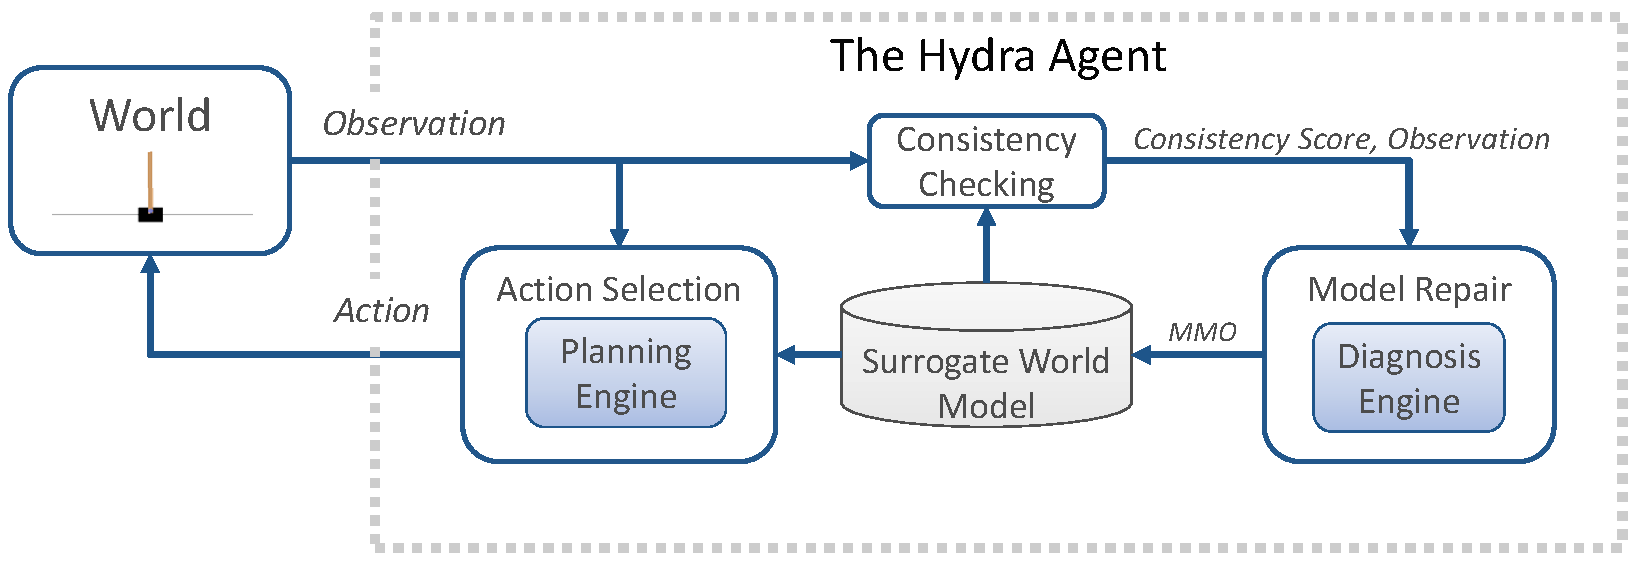
\includegraphics[width=\columnwidth]{hydra-cropped.pdf}
	\caption{An overview of the \hydra agent.}
	\label{fig:hydra-overview}
\end{figure}

\todo[inline,color=green]{[[Klenk: I think a gray box around all of the colored boxes here representing the \hydra agent would be helpful. The meta model does not perform actions.]]}




The model repair accepts the same input as the consistency checker as well as the output of the consistency checker. It suggests which changes should be made to the meta model so that it yields an updated surrogate model $\hat{E}$ that better predicts the observations. %to make the expected and observed states be more similar. 


The consistency checker uses $\hat{E}$ to predict the expected states according to the previously performed actions and compares them with the observed states. 

uses $\hat{E}$ to predict the expected states according to the previously performed actions and compares them with the observed states. 
\item \textbf{Meta model repair (MMR).} The model repair accepts the same input as the consistency checker as well as the output of the consistency checker. It suggests which changes should be made to the meta model so that it yields an updated surrogate model $\hat{E}$ that better predicts the observations. %to make the expected and observed states be more similar. 	

\item \textbf{Planner.} The planner accepts a state $\hat{s}\in\hat{S}$ in the surrogate model and generates a plan that, according to $\hat{E}$, will maximize the expected reward. Then, it outputs the action $\hat{a}\in\hat{A}$ to perform now according to this plan.
\item \textbf{Consistency checker (CC).} The consistency checker uses $\hat{E}$ to predict the expected states according to the previously performed actions and compares them with the observed states. 
\item \textbf{Meta model repair (MMR).} The model repair accepts the same input as the consistency checker as well as the output of the consistency checker. It suggests which changes should be made to the meta model so that it yields an updated surrogate model $\hat{E}$ that better predicts the observations. %to make the expected and observed states be more similar. 
illustrates \hydra's design. 
A \hydra agent tracks the actions it performs and observations it received to identify a state $\hat{s}$ in $\hat{E}$ that best represents the current state in $E$. 
Then, its \emph{Action Selection} component employs a \emph{planning engine} -- an automated planning algorithm -- to generate a plan that will maximize expected future reward. 

the current state of the environment

, and uses it as follows.
tracks the current state of the environment 


interacts with the environment $E$ 




\item \textbf{Action Selection.} This component tracks the current state of the world by keeping track of the performed actions and collected observations. Its role is to select which action to perform next. 
\item \textbf{Consistency Checking.} The consistency checking component matches the observed

uses $\hat{E}$ to predict the expected states according to the previously performed actions and compares them with the observed states. 
\item \textbf{Meta model repair (MMR).} The model repair accepts the same input as the consistency checker as well as the output of the consistency checker. It suggests which changes should be made to the meta model so that it yields an updated surrogate model $\hat{E}$ that better predicts the observations. %to make the expected and observed states be more similar. 	

\item \textbf{Planner.} The planner accepts a state $\hat{s}\in\hat{S}$ in the surrogate model and generates a plan that, according to $\hat{E}$, will maximize the expected reward. Then, it outputs the action $\hat{a}\in\hat{A}$ to perform now according to this plan.
\item \textbf{Consistency checker (CC).} The consistency checker uses $\hat{E}$ to predict the expected states according to the previously performed actions and compares them with the observed states. 
\item \textbf{Meta model repair (MMR).} The model repair accepts the same input as the consistency checker as well as the output of the consistency checker. It suggests which changes should be made to the meta model so that it yields an updated surrogate model $\hat{E}$ that better predicts the observations. %to make the expected and observed states be more similar. 
\end{itemize}




This environment surrogate model, denoted $\hat{E}$, is used to plan which actions to perform and detect when novelty is introduced by monitoring when the expected action outcomes differ from observations. 
A \hydra agent 



responds to detected novelty by modifying this surrogate model such that its predictions match the observations.


\begin{figure}
\centering
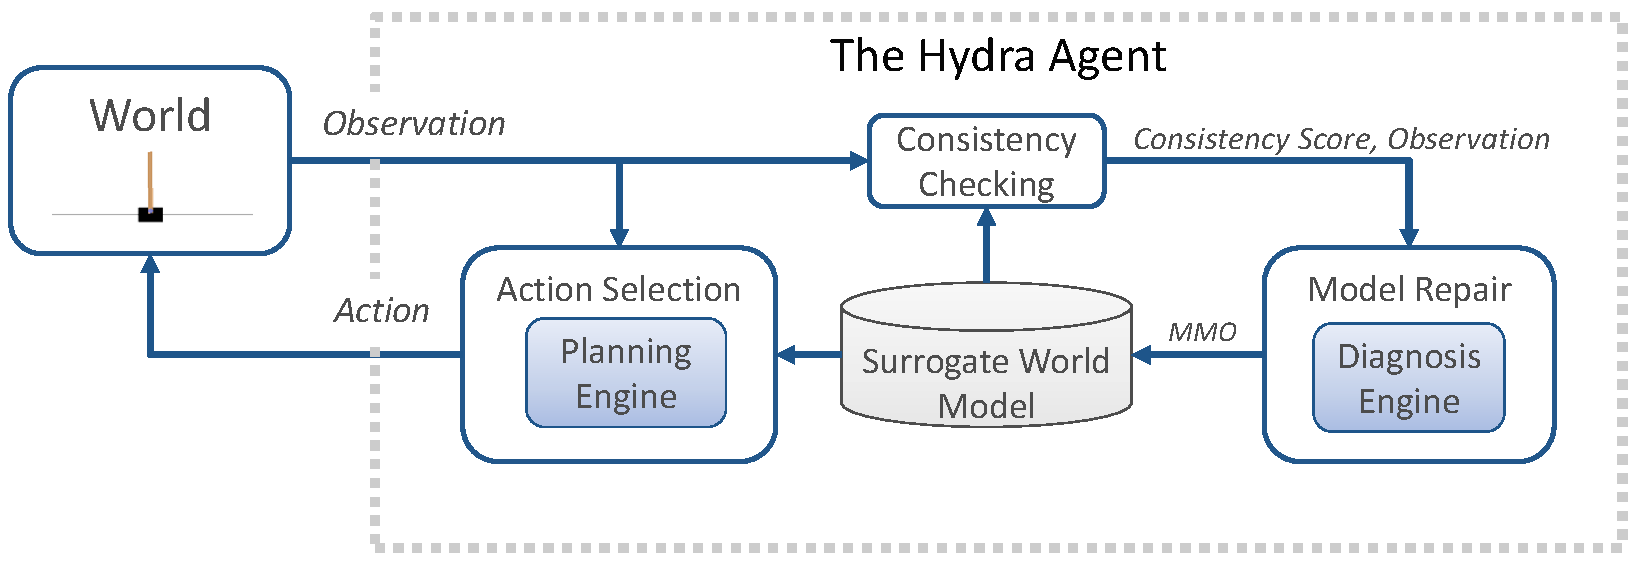
\includegraphics[width=\columnwidth]{hydra-cropped.pdf}
\caption{An overview of an \hydra agent.}
\label{fig:hydra-overview}
\end{figure}

Figure~\ref{fig:hydra-overview} illustrates \hydra's design. 

\hydra has three algorithmic components:
\begin{itemize}


\item \textbf{Action Selection.} This component tracks the current state of the world by keeping track of the performed actions and collected observations. Its role is to select which action to perform next. 
\item \textbf{Consistency Checking.} The consistency checking component matches the observed

uses $\hat{E}$ to predict the expected states according to the previously performed actions and compares them with the observed states. 
\item \textbf{Meta model repair (MMR).} The model repair accepts the same input as the consistency checker as well as the output of the consistency checker. It suggests which changes should be made to the meta model so that it yields an updated surrogate model $\hat{E}$ that better predicts the observations. %to make the expected and observed states be more similar. 	

\item \textbf{Planner.} The planner accepts a state $\hat{s}\in\hat{S}$ in the surrogate model and generates a plan that, according to $\hat{E}$, will maximize the expected reward. Then, it outputs the action $\hat{a}\in\hat{A}$ to perform now according to this plan.
\item \textbf{Consistency checker (CC).} The consistency checker uses $\hat{E}$ to predict the expected states according to the previously performed actions and compares them with the observed states. 
\item \textbf{Meta model repair (MMR).} The model repair accepts the same input as the consistency checker as well as the output of the consistency checker. It suggests which changes should be made to the meta model so that it yields an updated surrogate model $\hat{E}$ that better predicts the observations. %to make the expected and observed states be more similar. 
\end{itemize}







Most of \hydra's design is domain independent. To demonstrate this, we implemented \hydra on two very different benchmark domains --- Cartpole and \sbirds --- and highlight in this section the details of this implementation. In particular, we highlight which parts of our implementation are domain-independent and which parts are design choices that are domain specific. 


The first design choice is the modeling language used to define the surrogate environment model $\hat{E}$. 
Both domains require dealing with mixed discrete and continuous dynamics. In addition, \sbirds dynamics are governed by chains of reactions triggered by the agent's actions, unlike many other planning problems where most world changes are the direct result of agent actions. 
Due to these properties, we chose PDDL+~\cite{fox2006modelling} as our modeling language for $\hat{E}$. 
%PDDL+ allows modeling of the environment, its dynamics and behavior, as well as the agent's interactions with the environment. 
The defining characteristic of PDDL+ is the ability to model exogenous behaviour with discrete events and continuous processes.
Events apply discrete effects instantaneously, whereas processes apply changes continuously while their preconditions hold. The agent has no direct control over processes and events, and can only interact with exogenous activity indirectly. As noted above, \sbirds is overwhelmingly governed by processes and events, making PDDL+ an appropriate modeling language for our setting.  
In addition, PDDL+ generalizes many previously proposed planning languages, which simplifies supporting additional domains.




\begin{figure}
	\begin{center}
		% \begingroup
		\fontsize{8pt}{10pt}\selectfont
		\begin{verbatim}
			(:action pa-twang
			:parameters (?b - bird)
			:precondition (and
			(= (active_bird) (bird_id ?b))
			(not (angle_adjusted))
			(not (bird_released ?b)) )
			:effect (and
			(assign (vy_bird ?b) 
			(* (v_bird ?b) SIN(angle)))
			(assign (vx_bird ?b) 
			(* (v_bird ?b) COS(angle)))
			(bird_released ?b)
			(angle_adjusted)) )
		\end{verbatim}
		% \endgroup
		\caption{(Science Birds) Action releasing the bird from the slingshot, assigning initial velocities of the launched bird (approximations of sine and cosine functions are obscured).}
		\label{fig:action-pa-twang}
	\end{center}
\end{figure}



 standard well-known domain






% Domains description
\subsection{Domains}
The single persistent novelty setup and the novelty detection and response challenges can be studied on virtually any domain. In addition, the design of the agent is domain-independent, as well as most of its algorithmic components. 
However, we use the following two domains as running examples as well as a test bed for evaluating \hydra. 
For completeness, we provide a brief description of these domains.



% To demonstrate this, we implemented Hydra on two very different domains: \textbf{Cartpole} and \textbf{ScienceBirds}. 

\paragraph{Cartpole}






\paragraph{Science Birds}
This is a free version of the popular Angry Birds game developed for research purposes~\cite{renz2019ai}. 
In this single-player game, the player launches a finite set of birds in sequence
at a 2D structure made out of different material blocks and occupied by one or more pigs. The goal is to destroy all the pigs. 
Different birds and structures have different actions (e.g., yellow birds accelerate when the player taps the screen during flight) and properties (e.g., TNT objects explode when damaged by birds or other falling objects).
\sbirds is a challenging domain for AI agents due to the continuous action space and the large state space of resulting block configurations, and has maintained a yearly competition since 2012 \cite{renz2019ai}.


The agent interacts with the game through a server with the following API. After the level is loaded, the agent is given a list of objects with their outer hull polygons and a color-map that specifies the amount of each color inside the polygon\footnote{Raw pixels for the entire image are also available, but we do not use them in our system.}. 
The agent specifies shots by providing an $(X, Y)$ position to launch from and a time $t$ to tap the screen. The screen tap initiates actions based on bird type (e.g., a black bird will explode when tapped, a yellow bird will speed up, etc.). 
Thus, a state in this domain is the list of objects specified above and the possible actions are ``shoot at angle $\alpha$'' and ``tap''. 
Note that after shooting a bird the shoot action is not available until the target bird has become inactive and the level elements have settled. 
Similarly, after tapping a bird the tap action is not available until the next bird is released. 
In some time steps, there are no available actions, in which case a dummy ``no-op'' action is assumed.  
Shots that result in killing pigs or breaking blocks increase the score, which constitutes our reward function. 
A step constitutes shooting and potentially tapping a single bird. 
An episode here constitutes playing a single level. 
Playing a level starts with a finite set of birds that can be shot, and ends when either all pigs have been killed or when all the given birds were shot and have exploded. 
Examples of novelties in this domain are an increase in the force of gravity or an addition of a new type of bird with unique powers. 




In this section, we report on a small-scale demonstration of our PDDL+-based \hydra agent on the well-known balancing Cartpole domain. Cartpole is a classical RL benchmark domain in which a pole is connected to a cart and the task is to balance the pole in the upright position by pushing the cart either left or right.
There are multiple variants to the Cartpole domain. The variant we are using is defined as follows.
A state in this domain is represented by 4 state variables (velocities and positions of the cart and the pole).
In every step, the agent's action is to apply force to the cart in either left or right direction. 
An episode ends when either 200 steps have been performed or a limit is exceeded (i.e. pole angle or cart position). % [[TODO: min/max angle]]. 
Every step returns +1 reward, so the total reward for an episode is between 1 and 200. 
An example of a novelty in this domain can be as simple as a change in the mass of the pole or as difficult as adding wind or even an extra pole that interferes with the original pole. 
